\documentclass[conference]{IEEEtran}
\IEEEoverridecommandlockouts
% The preceding line is only needed to identify funding in the first footnote. If that is unneeded, please comment it out.
\usepackage{cite}
\usepackage{amsmath,amssymb,amsfonts}
\usepackage{algorithmic}
\usepackage{graphicx}
\usepackage{hyperref}
\usepackage{textcomp}
\usepackage{xcolor}
\def\BibTeX{{\rm B\kern-.05em{\sc i\kern-.025em b}\kern-.08em
    T\kern-.1667em\lower.7ex\hbox{E}\kern-.125emX}}
\begin{document}

\title{COVID-19 and NYC Crime}

\author{
\IEEEauthorblockN{Zhenzhou Xu}
\IEEEauthorblockA{\textit{New York University}\\
New York, USA \\
zx522@nyu.edu}
\and
\IEEEauthorblockN{Zete Dai}
\IEEEauthorblockA{\textit{New York University}\\
New York, USA \\
zd790@nyu.edu}
\and
\IEEEauthorblockN{Yinchu Zhao}
\IEEEauthorblockA{\textit{New York University}\\
New York, USA \\
yz6615@nyu.edu}
}

\maketitle


\section{Introduction}
Since the pandemic outbreak, people's daily lives change dramatically without any previous experience. As everything is transferred online, people's outdoor activities are severely restricted due to the highly contagious property of the COVID-19 Virus. For this new kind of social phenomenon, we are curious about how COVID-19 could ever change the criminal cases as people's outdoor activities are restricted. Therefore, with this question, we begin searching for data to validate the public safety trend under the pandemic.

We have made our code publicly available on GitHub.\footnote{\url{https://github.com/ZhenZhouXu/Data-analysis-project}}


\section{Problem formulation}
John MacDonald mentioned that the variance of crime rates across time is one of the oldest puzzles in the social sciences. Especially in a metropolis like New York City.~\cite{mac2020TheEffe} The crime rate could have rapid changes when various events happen. We want to find what changes the pandemic and the social distancing could cause to the crime in New York City. We want to know how COVID-19 affects the crime rate in each area in NYC? What age of criminals and what kind of crimes increase or decrease? How the unemployment rate caused by COVID could change the crime rate. And what the lockdown policy do to the changes in the crime rate.

Hypotheses are made that COVID-19 may cause the crime rate to increase due to the increasing unemployment rate, and it could also cause the crime rate to decrease due to the lockdown policy that further results in less outdoor activities.

\section{Related Work}
Exceptional phenomena, such as natural disasters and pandemics, could in a dramatic change in human actions. And COVID-19 is non-exceptional in this case, which not only leads to a massive loss of lives but also contributes to unprecedented loss of jobs and significant change in the distribution of crimes.

Abin Ojha stated in his study~\cite{ojha2020pandemic} that COVID-19 cases show a discrepancy in social classes, although there is a saying "The virus does not see race, caste, class, gender, region, religion, language, and border." COVID-19 affects the poor and marginalized members of society more seriously than others. Furthermore, in more seriously attacked areas, there shows a tendency that more people are suffering from unemployment and crimes.

From the study of David Abrams~\cite{abrams2020covid}, which assembled data from 25 large U.S. cities, it exists a national immediate drop in both criminal incidents and arrests most among drug crimes, theft, residential burglaries, and most violent crimes. However,  there is no decline in homicides and shootings, and there is even an increase in non-residential burglary and car theft.

Boman, John H and Gallupe, Owen have found out in their article~\cite{boman2020has} that the crime drop is being driven by decreases in minor offenses which are typically committed in peer groups. At the same time, serious crimes that are generally not committed with co-offenders (namely homicide and intimate partner violence) have either remained constant or increased. Their results are generally consistent with the one showed by David Abrams~\cite{abrams2020covid}.

More specifically, there are also studies directing at the influence of COVID-19 over hate crimes targeting Asian Americans. Gover, Angela R and Harper, Shannon B and Langton, Lynn published an article~\cite{gover2020anti} saying that Asian Americans reported a surge in racially motivated hate crimes involving physical violence and harassment. Throughout history, pandemic-related health crises have been associated with the stigmatization and “othering” of people of Asian descent.

It is shown that there are multiple works studying the relationship between COVID-19 and Crimes, which mainly focus on a national view of the entire United States. Meanwhile, there are few articles that specifically study the relationship in New York City.

\section{Methods}
To analysis the relationship between COVID-19 cases and the crimes in New York City, we need to find the appropriate datasets and grab the data we need. Then we use Hadoop and Spark to scale down large datasets and generate summary data, which are further processed by pandas to compose relationships between each dataset and finally visualized by Altair or Matplotlib. We analysis the COVID-19 report cases and the timeline of the influence events to make the connections with our data.

\subsection{COVID-19 Cases}
We download the Data Table for Case Daily Trends in New York City from the CDC COVID Data Tracker. It tracked the case count from January 21st to December 8th. 

\subsection{Unemployment Rate}
From the report wrote by Sandra Ajimotokin, The Effects of Unemployment on Crime Rates in the U.S.~\cite{ajimotokin2015effects}, We can hypothesize there would be a positive correlation between unemployment and crime rate. The COVID in New York City caused heavy restrictions and social distancing, making many people lost their job since stores were closed. We want to see how the unemployment rate and the social distancing under COVID policies affect the crime in NYC. We found the unemployment rate for each borough on the website of the Department of Labor. The dataset recorded the unemployment rate for all 62 counties including the 5 boroughs in New York City since 1990. We separate data for different boroughs to help us analyzing in detail.

After getting the summary data of unemployment in different boroughs, pandas are used to transform these wide-form data to long-form data, which are later concatenated together. Besides, in order to visualize the unemployment data in different boroughs, we need to acquire the geographical data of five boroughs in New York City. The geographical data of different boroughs of New York City is collected from NYC Open Data~\cite{nyc2020boroughboundaries}. Finally, \verb|transform_lookup| is used to join the unemployment data with the geographical data and \verb|mark_geoshape| is used for displaying the unemployment distribution in different boroughs.



\subsection{Crime}
There are various kinds of crimes happening every day in New York City. We try to specify several important crime categories and do the comparison of these crimes with date in order to figure out how significant event like NYC-lockdown policy and COVID 19 cases affects the crimes cases in total and crime cases of each category. We also compare different age-group crime cases to find out how different people in each age group act differently towards this crisis.

\subsubsection{Age Group}
Different age groups may acts differently towards this crisis for the reason that the news propaganda of old people's vulnerability to COVID 19. Younger people may have stronger immunity and hence they may not restrict their outdoor activity. To validate this hypothesis, we extract data from the NYPD arrest data set and use spark to summarize the data over each age group. Finally, we draw the graph of criminal cases and the date. Compare different age group cases variation over time.

\subsubsection{Hate Crime}
Ever since the beginning of the pandemic, there are lots of news going on about hate crimes targeting Asians is rising in NYC~\cite{irene2020hatecrimes}. Therefore, this report wants to find out if it is the truth and also explores the changes in hate crimes targeting different races before and during the COVID-19.

The data are required from a data set called NYPD Hate Crimes~\cite{NYPD2020hatecrimes} from NYC Open Data. Steps performed to clean and integrate the data is as listed below:
\begin{itemize}
    \item Checking for duplicates in Full Complaint ID and Arrest Id which must be unique.
    \item Checking for invalid/null value in several columns like Record Create Date,	Complaint Precinct Code, County, etc..
    \item Clustering on different columns (mainly Bias Motive Description) about the rows with the same intended values but different actual values due to inconsistency caused by human input.
    \item Filter out the rows which have inconsistent Record Create Date and Arrest Date.
    \item Manually add the header to the output file generated otherwise multiple headers will be added to the file if it's done by Spark SQL (each thread will add one header). 
    \item Conditionally select rows where Bias Motive Description is ANTI-WHITE, ANTI-ASIAN, ANTI-BLACK, ANTI-JEWISH, and ANTI-HISPANIC and group and sort them by Record Create Date.
\end{itemize}

After getting the summary data, Altair is used to transform this wide-form data to long-form data. The final data is visualized together with the unemployment data.

The challenges faced in this dataset are the followings:
\begin{itemize}
    \item It is not sure that some records (rows) should be excluded or not because it is sometimes valid to have null values in certain columns.
    \item Sometimes finding rows with invalid values is tedious unless coming up with a meticulous regular expression.
\end{itemize}

\subsubsection{Shooting}
Shooting is always a serious crime. Since the social distancing and other COVID regulations, people are not going out so often as before the pandemic. We would like to see how these changes in people's daily life could change the shooting case in New York City.

The dataset was download from NYC Open Data from the link in the NYPD website. Steps performed to clean and integrate the data is as listed below:
\begin{itemize}
    \item Remove all lines where Date type is not Date.
    \item Checking for duplicates Date which must be unique.
    \item Sort the rows by Date with the format of MM/DD/YY.
    \item Clustering on unique dates to have the shooting count for each day.
    \item Format the output document with 2 columns (Date, Count).
\end{itemize}
Then we used Altair to making further visualization with the unemployment rate.
Items below are the challenges that we faced:
\begin{itemize}
    \item There are other events happening at the same time that we could not control variables in this research.
    \item The changes in daily counts are changing rapidly. It is hard to match our result with prediction.
\end{itemize}		

\subsubsection{Burglary}
Burglary refers to the crime of illegally breaking and entering any structure with the intent to commit any crime inside like theft or larceny. Due to the effects of the pandemic and the lockdown policy, people are running out of their livelihood without any assistance in the beginning. Will the crime rate increase dramatically for this reason? How will the pandemic affect burglary crime cases or crime rates before and after the pandemic? We will compare the counts of burglary to the date to see the actual effect of the pandemic.



\subsubsection{Traffic Violation}
Traffic violations occur when the driver violates the laws that regulate vehicle operation on streets and highways. As the significant event-New York lockdown policy executed, we think people's outdoor activity may significantly decrease. So the traffic violation cases may significantly decrease as well. This is an important category of crimes to estimate the hypothesis that people will restrict their willingness to travel or driving when the pandemic occurs for their serious damage to public health.

The dataset we used for Age group, Burglary and Traffic Violation was from arrest data in NYPD website in 2020 from January to September. The following steps are performed to clean, cluster and plot the data:
\begin{itemize}
\item Check for NULL value in each row
\item Used nearest neighbour to find out crime category that has similar meaning
\item integrate the data according to each category of crimes, age group and total number of cases.
\item we find out that some data fluctuated too quickly to observe the data trend, Rolling means was used to flatten the variation of the data and made the data be easier to be observed.
\end{itemize}
\section{Results}

\subsection{Unemployment Rate}
 Figure~\ref{fig:unemployment_2020} shows the trend of unemployment rate data collected from New York state website~\cite{newyork2020unemployment} in five boroughs of New York City (The Bronx, Brooklyn, Manhattan, Queens, and Staten Island) in 2020. It is shown that different areas are under different impact of the unemployment caused mainly by COVID-19. The poorest borough Bronx that also has the highest crime rate is under most severe attack by the unemployment, which reflects the discrepancy in social classes.

\begin{figure}[ht!]
    \centering
    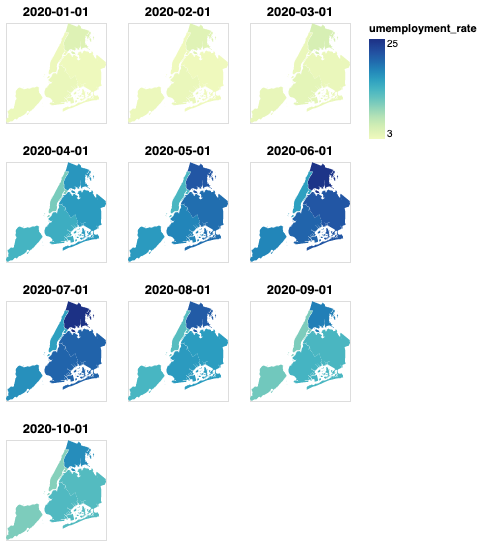
\includegraphics[width=\linewidth]{images/unemployment_boroughs_2020.png}
    \caption{New York City Unemployment Rate in 2020}
    \label{fig:unemployment_2020}
\end{figure}

\subsection{Crime}

\subsubsection{Total Crime Cases}
Figure~\ref{fig:totalCrimeCases_2020} shows the total crime cases change in each Borough from January to September from NYC open data of arresting data in 2020. As we can see, when the lockdown policy published on March, the total crime cases dropped dramatically and this policy was very effective due to outdoor activities was restricted; However, there was a sudden rise from March to June. Several reasons may contribute to this trend during that period. After plotting the data of each borough in line format,  Figure ~\ref{fig:BoroughLineGraph} clearly shows that Manhattan crime cases rose rapidly from May to June.


\begin{figure}[ht!]
    \centering
    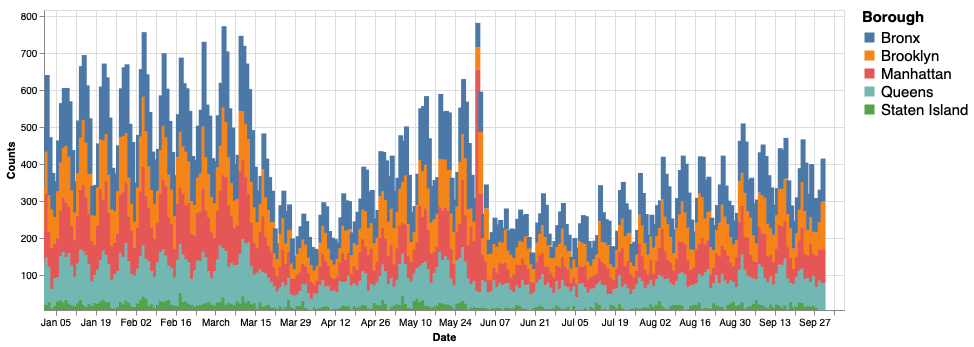
\includegraphics[width=\linewidth]{images/totalCrimeCases.png}
    \caption{New York City total crime cases in each borough in 2020}
    \label{fig:totalCrimeCases_2020}
\end{figure}

\begin{figure}[ht!]
    \centering
    \includegraphics[width=\linewidth]{images/BoroughLineGraph.png}
    \caption{NYC crime cases line graph in each borough in 2020}
    \label{fig:BoroughLineGraph}
\end{figure}

\subsubsection{Age Group}
Figure ~\ref{fig:AgeGroup_2020} shows the crime cases trend before and after the pandemic.  From January to March, the criminal cases were stable and after the release of the lockdown policy, the crime cases over each age group were decreasing dramatically. But except for the age group of 65+,  other age groups all rise suddenly from March to June. We think people over 65 are more concerned about their health and follow the guided rules of staying at home. So the cases dropped and stay constant with little difference from March to September. Other age groups all rise suddenly in the middle of the time.

\begin{figure}[ht!]
    \centering
    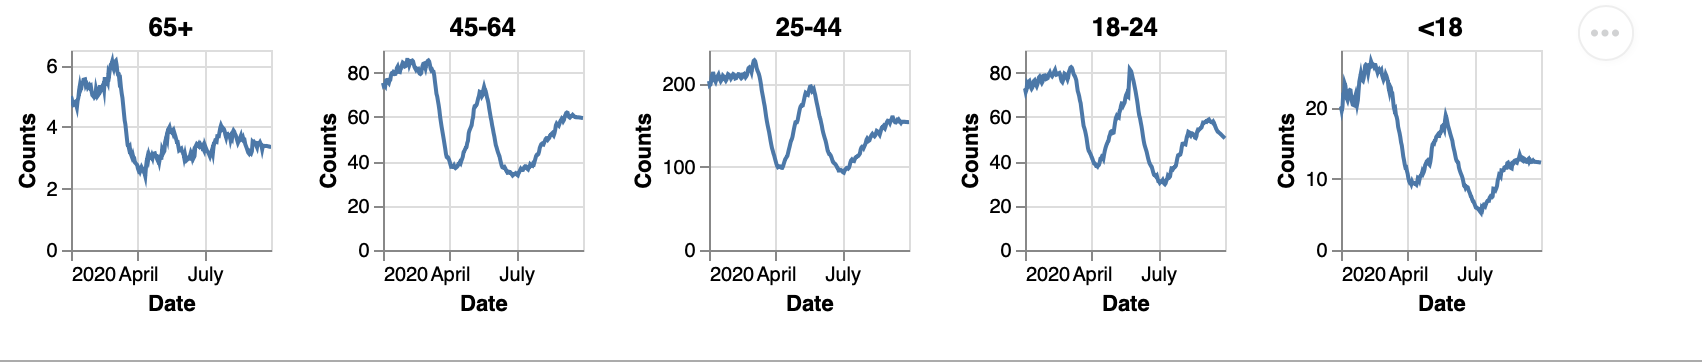
\includegraphics[width=\linewidth]{images/AgeGroup.png}
    \caption{Crime cases trend over each age group in 2020}
    \label{fig:AgeGroup_2020}
\end{figure}

\subsubsection{Hate Crime}
Figure~\ref{fig:hate_crime} shows the trend of the hate crimes data collected from NYC open data~\cite{NYPD2020hatecrimes} targeting different races in 2019 and 2020, compared with the trend of the unemployment rate in the background (the red line).
The figure~\ref{fig:hate_crime} clearly shows that there is a rise in the hate crimes targeting Asians at the beginning of the pandemic. However, the overall number of hate crimes seems to go down with the ongoing pandemic which might result from less outdoor activities.

\begin{figure}[ht!]
    \centering
    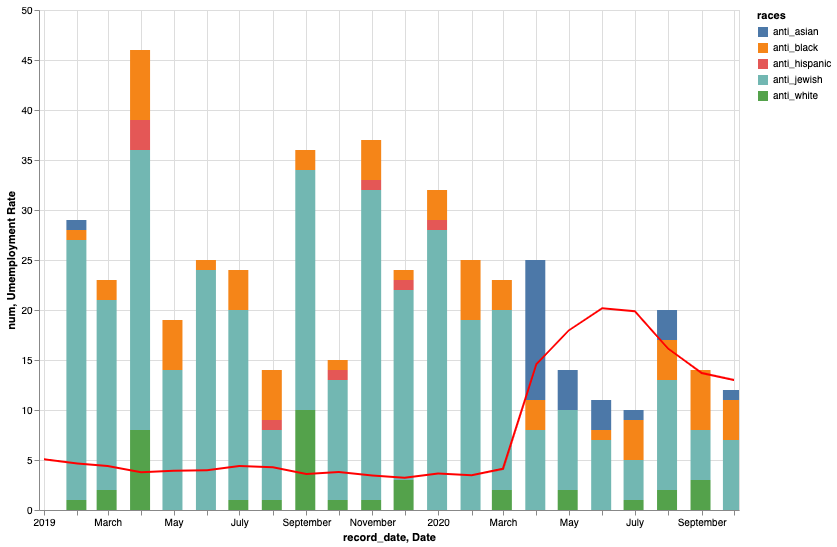
\includegraphics[width=\linewidth]{images/hate_crime.png}
    \caption{New York City Hate Crimes Compared with Unemployment Rate}
    \label{fig:hate_crime}
\end{figure}

\subsubsection{Shooting}
Figure~\ref{fig:Shooting&UER} is the graph of the unemployment rate and the shooting cases changes by time. We gathered the shooting cases in New York City on the NYPD website from 2019 to 2020. The unemployment rate is the red line and the blue blocks are the daily shooting cases. The figure shows the shooting cases are not necessarily affected by the unemployment rate before the pandemic. But there is an apparent increase in shooting cases when the unemployment reaches the top in June. At the same time, the Black Lives Matter protests are also causing chaos in June. So we can not conclude that the unemployment rate caused by the pandemic is changing the shooting cases.



\begin{figure}[ht!]
    \centering
    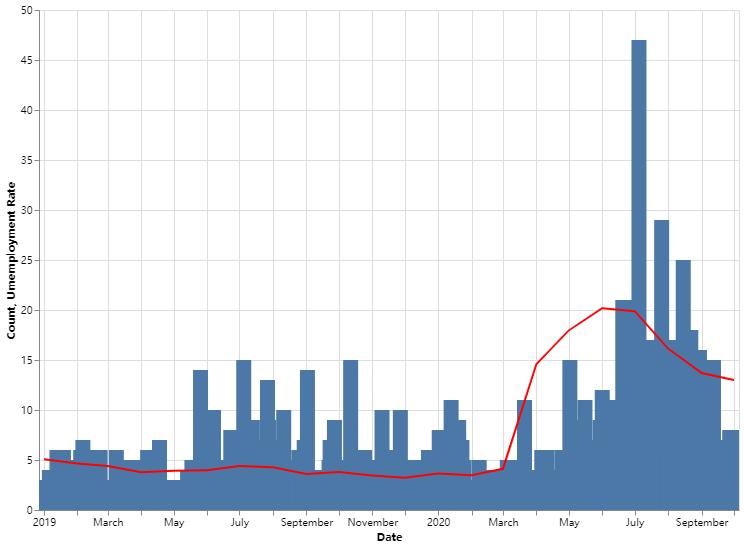
\includegraphics[width=\linewidth]{images/Shooting&UER.png}
    \caption{New York City Shooting Cases Compared with Unemployment Rate}
    \label{fig:Shooting&UER}
\end{figure}

\subsubsection{Burglary}
Figure ~\ref{fig:TrafficAndBurglary} shows sudden increase of burglary from March to June. Several reasons may be counted for this trend. As people staying at home and running out of livelihood, they may eager to commit crimes and steal. On the other hand, there was a protest march from May to June in Manhattan. The outdoor activities suddenly increase dramatically during that time. So crime cases will increase for this reason.


\begin{figure}[ht!]
    \centering
    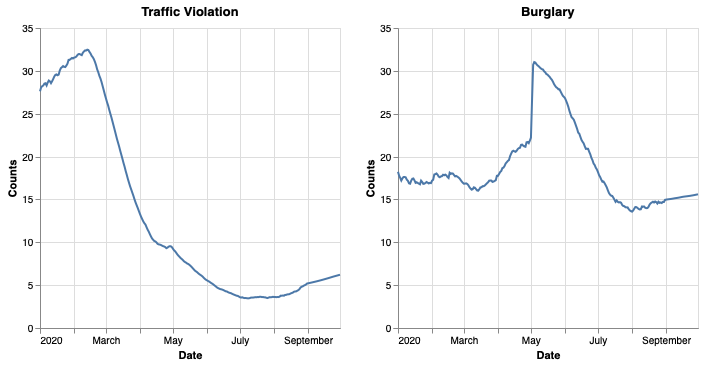
\includegraphics[width=\linewidth]{images/TrafficAndBurglary.png}
    \caption{Traffic violation and Burglary cases in 2020}
    \label{fig:TrafficAndBurglary}
\end{figure}

\subsubsection{Traffic Violation}
Figure ~\ref{fig:TrafficAndBurglary} shows Traffic violation is dropping dramatically in New York city, as the lockdown policy published, Many restaurants and markets were restricted for opening time. People were less likely to drive or go outside as we observe from this graph.

\section{conclusion}
Overall, COVID 19 has a significant impact on numerous aspects of people's daily lives. As shown in the visualization, the pandemic was effective over the unemployment rate, total crime cases, and specific categories of crimes.

In the unemployment rate:
COVID-19 has shown its enormous impact on unemployment in different areas, while the poor suffer the most in this situation. There also shows a pattern that boroughs with higher crime rates are affected more by the pandemic leading to more job losses.

In total crime cases:
COVID-19 and the lockdown policy was quite effective for the total crime cases; However, as the unemployment rate was increasing, people were running out of their livelihood as well as the damage of mental health when people keep staying at home. Crime cases rose up rapidly to the climax in June.

In specific categories of crimes:
There is a rise in the hate crimes targeting Asians at the beginning of the pandemic, while the overall number of hate crimes goes down with the ongoing pandemic which might result from less outdoor activities.
There is a small impact on the shooting case by COVID. Since other violations happened at the same time that are not caused by COVID, we can not conclude that COVID affects the cases of shooting crime.
Burglary crime cases clearly show the impact of the high unemployment rate on public safety. Traffic violation cases show the effectiveness of lock-down policy over the outdoor activities of people. Each crime category was closely related to each other and revealed what was happening in New York City.

\bibliographystyle{IEEEtran}
\bibliography{biblography}

\end{document}
